\documentclass{article}

\usepackage{amsmath}
\usepackage[utf8]{inputenc}
\usepackage[T1]{fontenc}
\usepackage{parskip}
\usepackage{graphicx}
\usepackage{geometry}
\usepackage{epstopdf}
\usepackage{siunitx}
\usepackage{eurosym}
\usepackage{listings}
\usepackage{courier}
\usepackage[shortlabels]{enumitem}

\begin{document}
\section*{C++ Programming project plan - Micro Machines 5}
{\large Juuso Korvuo}\\
{\large Lauri Kurkela}\\
{\large Lauri Nyman}\\
{\large Henry Räbinä}

\subsection*{Overview}

The goal of this project is to create a top-down racing game inspired by Micro Machines. The objective of the game is to finish a specified amount of laps before opponent players. The levels consist of roads and other material types which the players can drive on, and checkpoints which have to be reached in a certain order. In addition, the levels include physical objects (e.g., rocks, railings) with which the players can collide. The players may also collide with each other.

The initial plan is to use cars as the vehicle types, and plan the levels accordingly. Additional vehicle types and levels for them may be added if we have enough time. Other possible additions are weapons (for example mines, missiles or other types of guns) for disrupting other players, a level editor for easy level creation, AI and online multiplayer.

The game will have a menu screen, consisting of at least a start game button, an options menu and an exit button. Possible options are changing the control scheme of the players and the sound settings (if sounds are implemented). Our plan is to implement the actual gaming screen such that the whole racing track is visible at the same time. This means that the screen will not be "moving" with the player. We will use this approach beacause all the players will need to see themselves on the track at the same time.

The driving physics of the vehicles and collision detection will be handled by the Box2D physics engine. The user interface and graphics will be drawn using SFML.

\subsection*{Rudimentary class structure and description}
\subsubsection*{Level}
The level class will contain a matrix of block types, where each element of the matrix defines the material of the road at some coordinates. For example, a 1000x1000 pixel level could be defined by a 100x100 matrix, where each element corresponds to a 10x10 pixel block of the level. This allows easy queries to ask what the material of the ground is at some coordinates, and the vehicle physics can be adjusted accordingly (decrease friction on ice, decrease max speed on mud, etc.). In case the matrix idea turns out to be unfeasible, we may also construct the levels using Box2D shape objects (chain shapes etc.). The level will also contain a list of all physics objects in it (objects which use collision mechanics). A file from which the level is loaded will contain the values of the block matrix and the necessary details about the physics objects.

\subsubsection*{PhysicsObject}
The objects in the level which use features from the Box2D library will be physics objects. The purpose of this class is to tie the body of the object created using Box2D to the graphics created using SFML, to allow easy drawing of the objects. Vehicles and static obstacles such as rocks inherit from this class.

\subsubsection*{Vehicle, Car, Boat etc.}
Vehicle is an abstract class which defines some common properties and methods of all vehicles (asking coordinates, for example). The child classes have different values for vehicle type specific constants, such as max speed and friction. We believe that this is the best approach because all the different types of vehicles work according to the same principle. Thus, there is no need to make a completely individual class for each vehicle type.

\subsubsection*{StaticObstacle}
Static obstacles are objects which have collision properties and are placed on the level. These could include rocks, trees and so on. The idea is that static obstacles do not move under collisions, so the players have to dodge them.

\subsubsection*{Player}
The player class represents the player of the game. It will contain information about the player, such as their name, control scheme and currently used vehicle.

\begin{figure}[!ht]
\centering
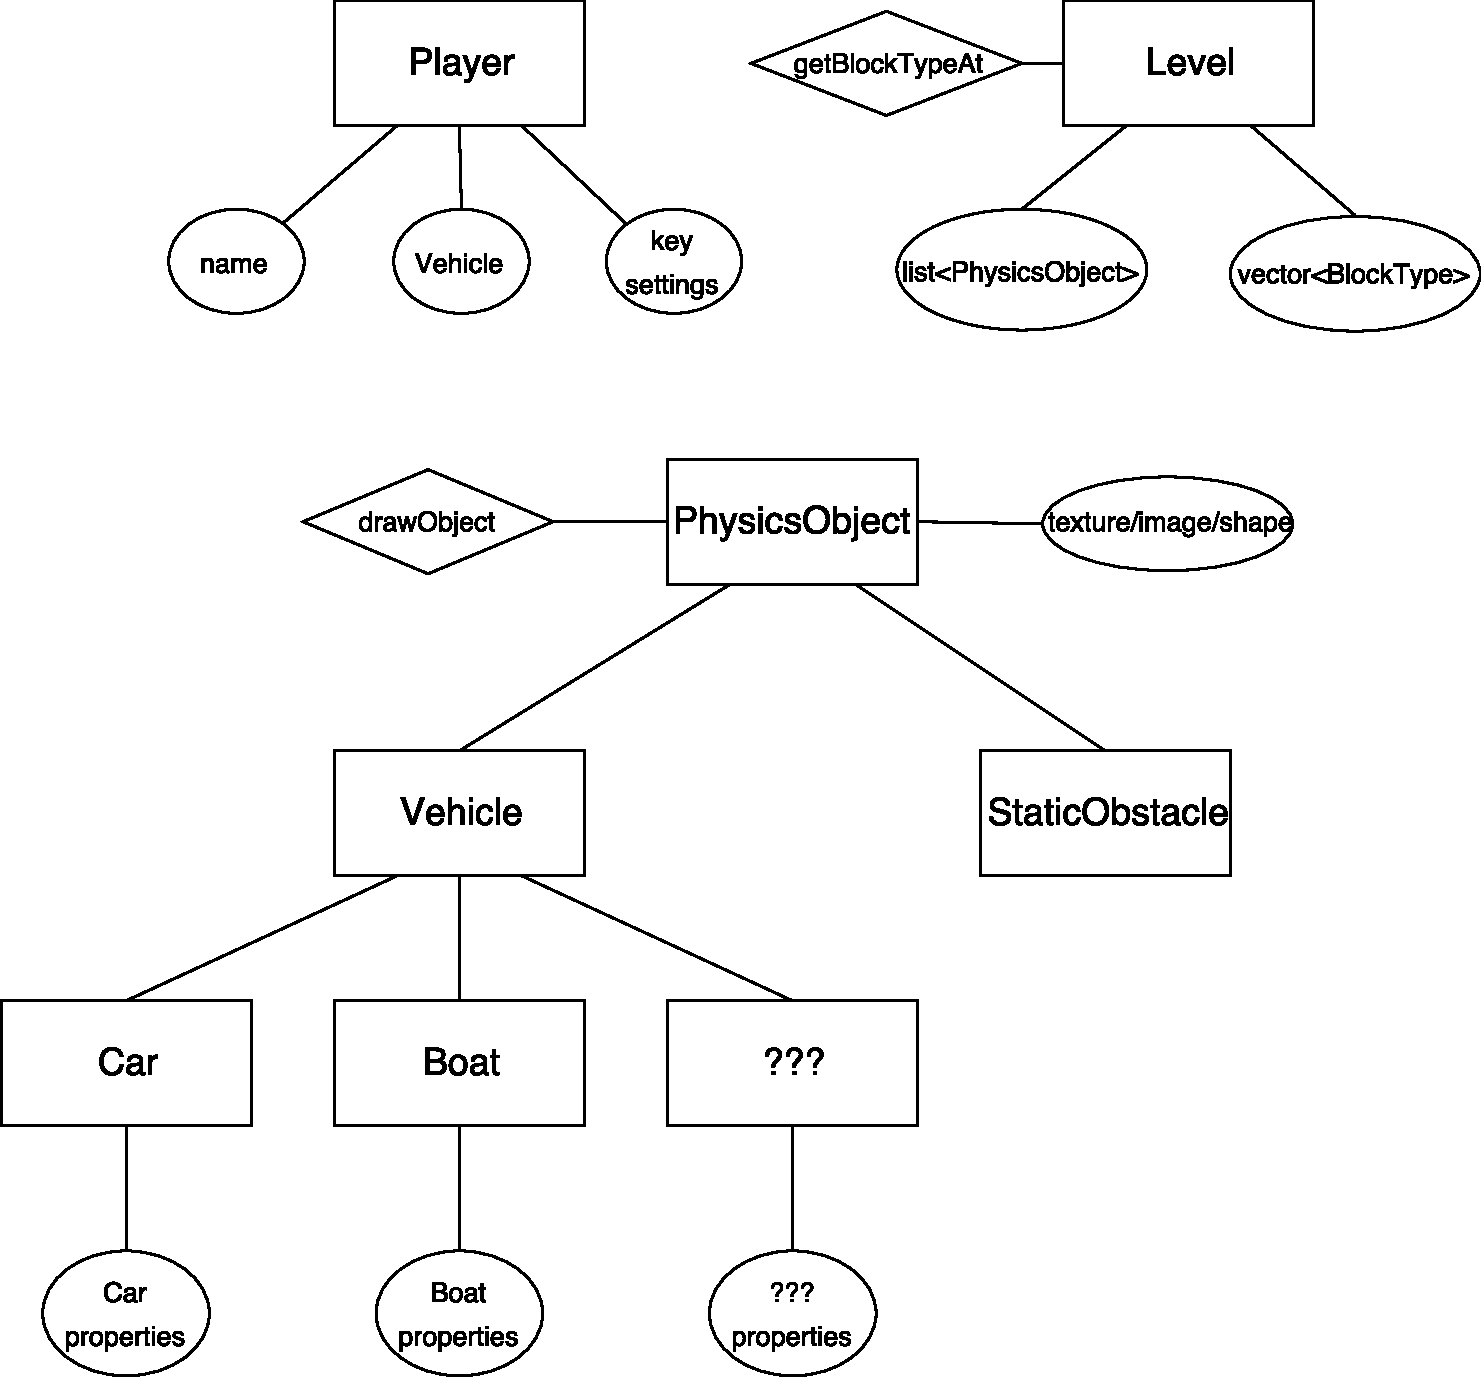
\includegraphics[width=\textwidth]{classes.pdf}
\caption{Rudimentary class structure. Rectangles describe classes, diamonds describe their methods and ellipses describe variables or information stored within the class. Functions.cpp contains miscellaneous functions for handling menu windows and game events.}
\end{figure}

\subsection*{Preliminary schedule}
Week 46: Working on the project plan. Getting started with the implementation of the different classes, the menu window and the makefile.

Week 47: Continuing with the implementation of the classes

Week 48: Mid-term meeting: a working prototype
\begin{itemize}
\item Player class implemented with one vehicle class
\item Level class implemented with one level
\end{itemize}

Week 49: Finishing touches to the basic classes. Completing the project documentation

Week 50: Continuing with week 49 tasks if necessary. If there is time, we will try to implement a level editor and an online multiplayer option for the game.

\subsection*{The group and distribution of roles}
The group will aim to meet at least once every week to discuss progress and plan ahead. We will also communicate using Telegram to discuss urgent matters.

The roles will probably change over the course of the project, but the first tasks are distributed as follows:

Juuso will start working on implementing the vehicle classes and the driving physics.

Lauri K. will create the makefile(s) and structure the project directory.

Lauri N. will start working on the Level class.

Henry will start working on the menus.

\end{document}
